\documentclass{article}

\usepackage{graphicx}
\usepackage{tikz}
\usepackage{tikzsymbols}
\usetikzlibrary{calc,patterns,shapes.geometric}
\pagestyle{empty}
\usepackage[margin=0pt]{geometry}
\geometry{papersize={14in,12in}}

\def\centerarc[#1](#2)(#3:#4:#5){\draw[#1] ($(#2)+({#5*cos(#3)},{#5*sin(#3)})$) arc (#3:#4:#5);}

\begin{document}
	\begin{figure}
		\centering
		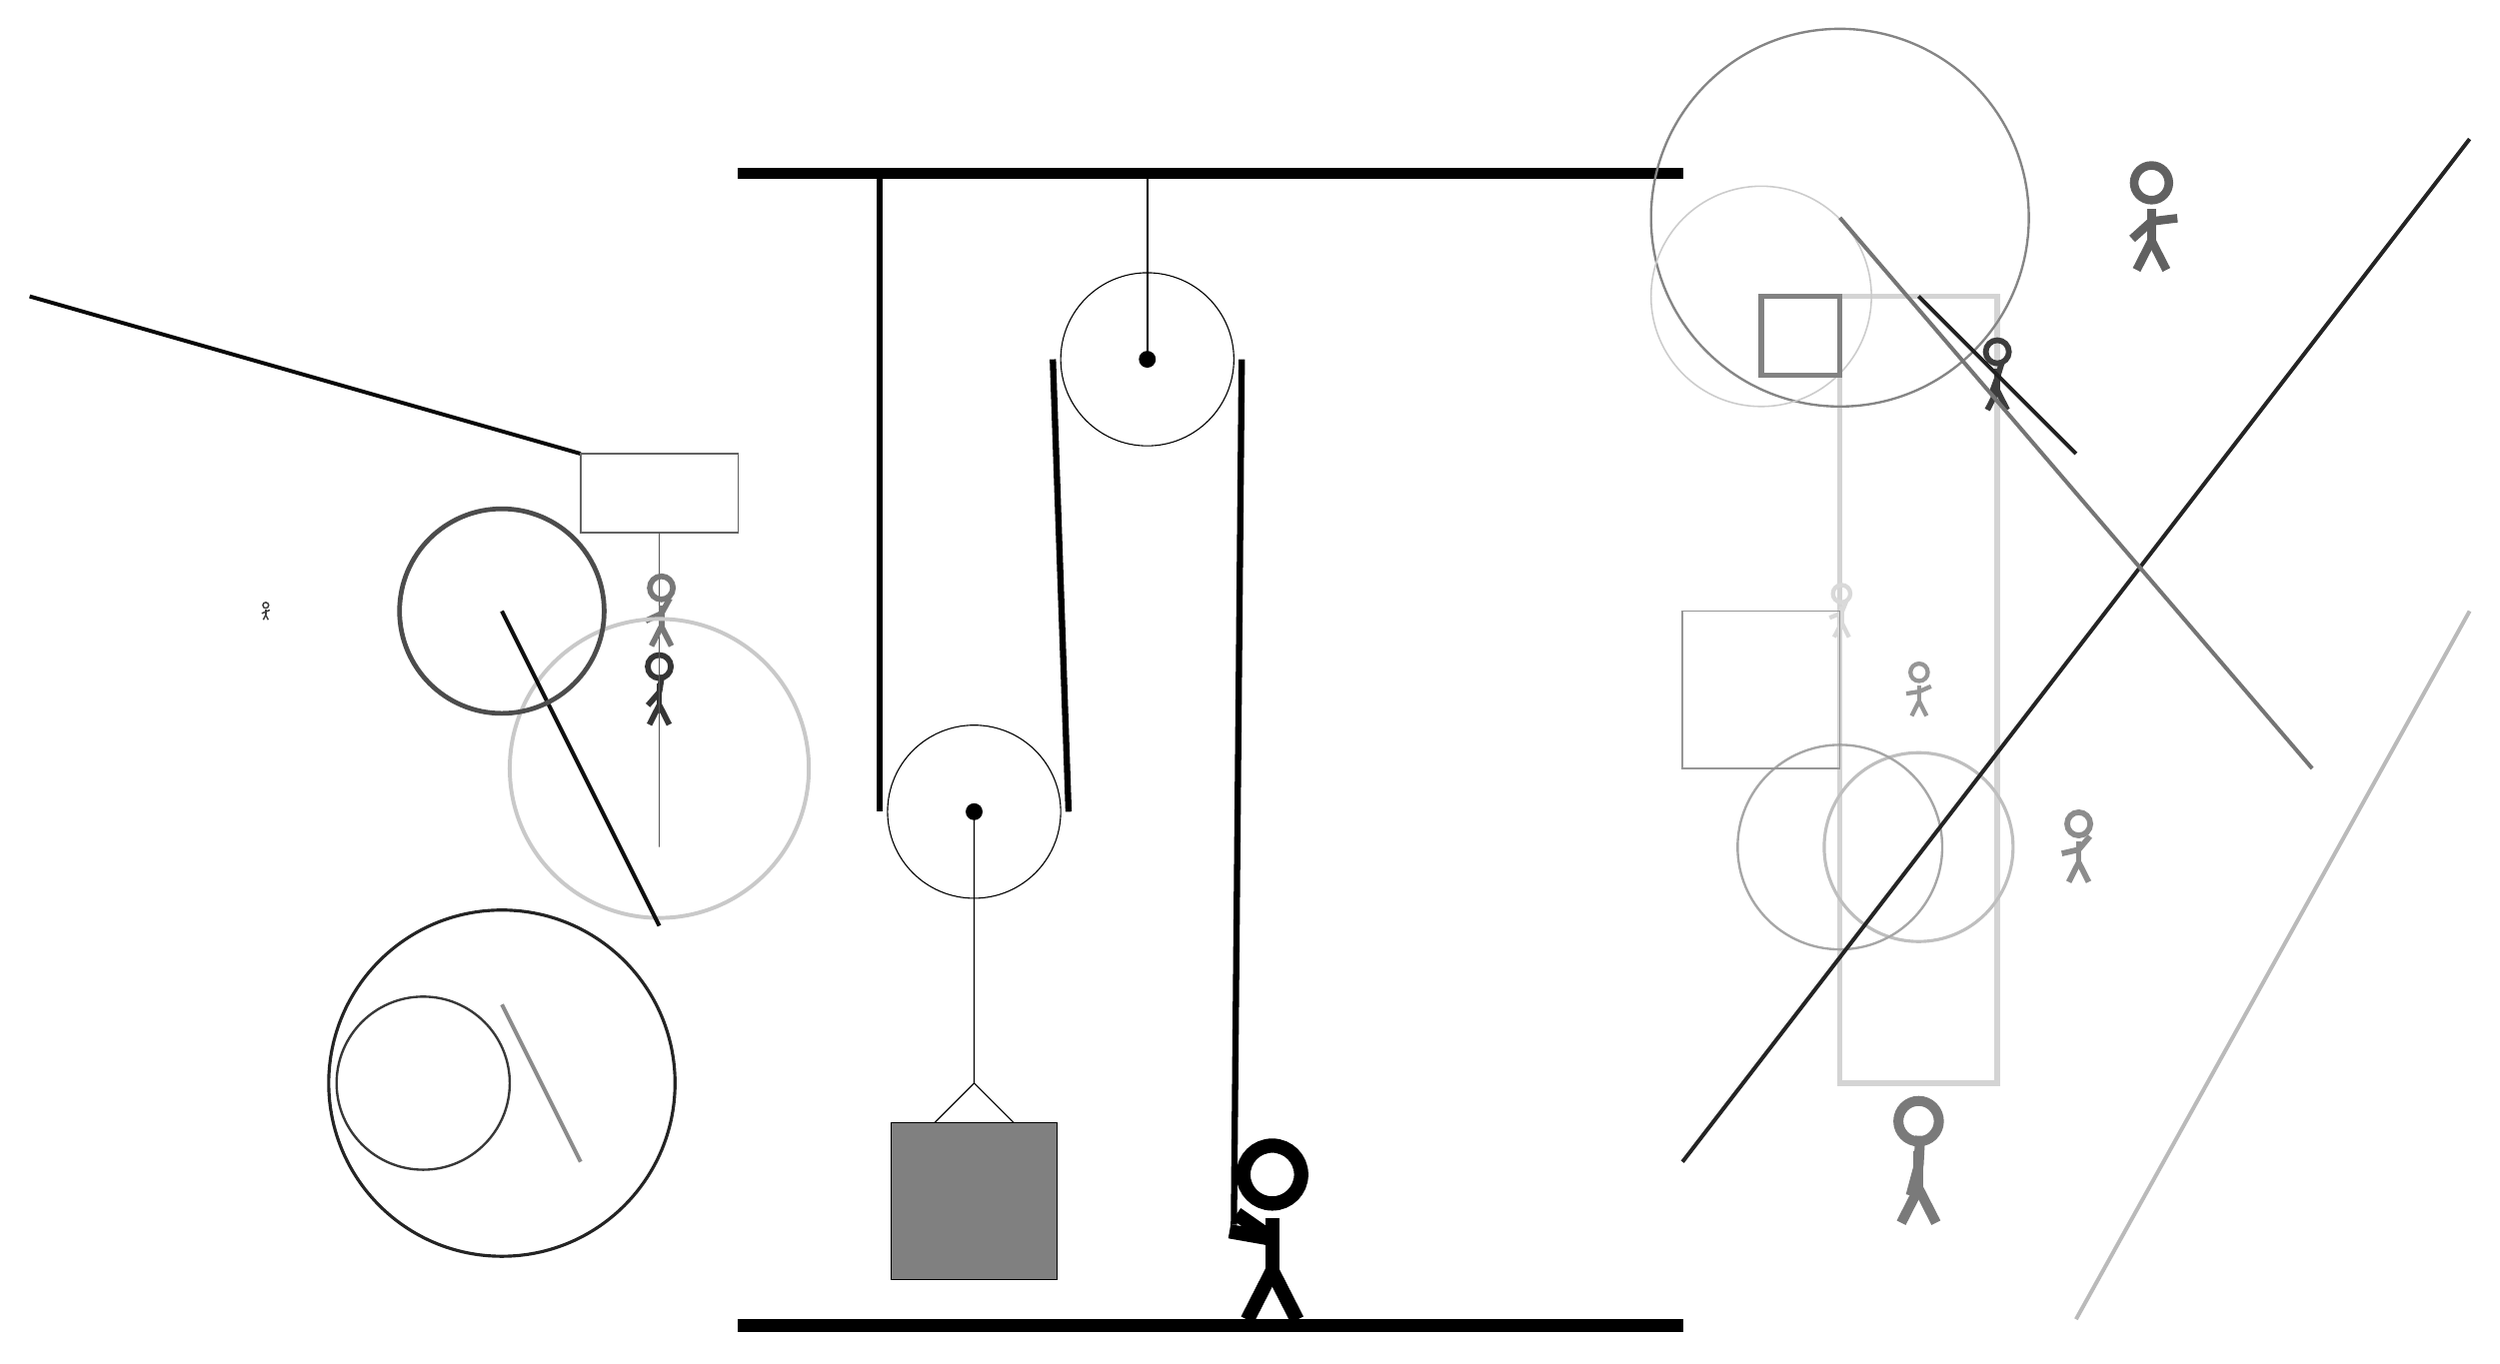
\begin{tikzpicture}
			%%%%% START %%%%%
			
			\draw[fill=black] (-2, 11.5) rectangle (10, 11.625);
			
			\draw (3.2, 9.2) circle (1.1);
			\draw[fill=black] (3.2, 9.2) circle (0.1);
			\draw[thick] (3.2, 9.2) -- (3.2, 11.5);
			
			\node[line width=0.2mm, color=black!79] at (-3, 5) {\Strichmaxerl[4][49][81]};
			
			\draw[line width=0.7mm, color=black!17] (12, 0) rectangle (14, 10);
			\draw [line width=0.3mm, color=black!48](12, 11) circle (2.4);
			\draw[line width=0.5mm, color=black!97](-4, 8) -- (-11, 10);
			
			\draw [line width=0.2mm, color=black!20](11, 10) circle (1.4);
			\draw [line width=0.4mm, color=black!86](-5, 0) circle (2.2);
			\draw[line width=0.2mm, color=black!61] (-2, 8) rectangle (-4, 7);
			\draw[line width=0.2mm, color=black!66] (-3, 7) rectangle (-3, 3);
			\draw [line width=0.4mm, color=black!25](13, 3) circle (1.2);
			\node[line width=0.3mm, color=black!15] at (12, 6) {\Strichmaxerl[3][22][68]};
			\node[line width=0.4mm, color=black!76] at (14, 9) {\Strichmaxerl[4][70][73]};
			\draw [line width=0.3mm, color=black!35](12, 3) circle (1.3);
			\node[line width=0.5mm, color=black!53] at (-3, 6) {\Strichmaxerl[4][25][61]};
			
			\draw [line width=0.5mm, color=black!21](-3, 4) circle (1.9);
			\draw[line width=0.5mm, color=black!27](15, -3) -- (20, 6);
			\draw[line width=0.5mm, color=black!86](10, -1) -- (20, 12);
			\draw[line width=0.5mm, color=black!94](-5, 6) -- (-3, 2);
			\draw [line width=0.2mm, color=black!71](-6, 8) circle (0.0);
			\node[line width=0.4mm, color=black!77] at (-8, 6) {\Strichmaxerl[1][23][22]};
			\draw [line width=0.3mm, color=black!78](-6, 0) circle (1.1);
			\draw[line width=0.5mm, color=black!87](15, 8) -- (13, 10);
			\node[line width=0.2mm, color=black!52] at (13, -1) {\Strichmaxerl[7][75][87]};
			\node[line width=0.2mm, color=black!62] at (16, 11) {\Strichmaxerl[6][42][7]};
			\draw[line width=0.5mm, color=black!45](-4, -1) -- (-5, 1);
			\node[line width=0.5mm, color=black!45] at (15, 3) {\Strichmaxerl[4][13][50]};
			\draw[line width=0.2mm, color=black!41] (10, 4) rectangle (12, 6);
			\node[line width=0.4mm, color=black!41] at (13, 5) {\Strichmaxerl[3][9][24]};
			\draw[line width=0.5mm, color=black!54](12, 11) -- (18, 4);
			\draw[line width=0.7mm, color=black!49] (11, 10) rectangle (12, 9);
			\draw [line width=0.6mm, color=black!70](-5, 6) circle (1.3);
			
			\draw (1, 3.45) circle (1.1);
			\draw[fill=black] (1, 3.45) circle (0.1);
			
			\draw (1, 3.45) -- (1, 0.0) -- (0.5, -0.5);
			\draw (1, 0.0) -- (1.5, -0.5);
			\draw[fill=black!50] (-0.05, -0.5) rectangle (2.05, -2.5);
			
			\draw[line width=0.8mm] (-0.2, 11.5) -- (-0.2, 3.45);
			\centerarc[line width=0.8mm](1, 3.45)(180:360:1.2000000000000002);
			\draw[line width=0.8mm](2.2, 3.45) -- (2.0, 9.2);
			\centerarc[line width=0.8mm](3.2, 9.2)(0:180:1.2000000000000002);
			\draw[line width=0.8mm](4.4, 9.2) -- (4.3, -1.8);
			
			\node at (4.7, -1.9) {\Strichmaxerl[10][-35][170]};
			
			\draw[fill=black] (-2, -3) rectangle (10, -3.15);
			
			%%%%% END %%%%%
		\end{tikzpicture}
	\end{figure}	
\end{document}